%!TEX root = teaching_statement_example_yw.tex
%!TEX program = lualatex

\documentclass{tufte-handout}

\geometry{
    top=0.75in, % top margin
    bottom=0.75in, % bottom margin
    left=0.75in, % left margin
    textwidth=4.95in, % main text block
    marginparsep=0.3in, % gutter between main text block and margin notes
    marginparwidth=2in % width of margin notes
}

\usepackage{lastpage}
\usepackage{xfrac}
\pagestyle{fancy}
\fancyhf{}
\renewcommand{\headrulewidth}{0pt}
\renewcommand{\footrulewidth}{0pt}

\usepackage[T1]{fontenc}
% load babel here
\usepackage[p,osf]{cochineal}
\usepackage[varqu,varl,var0]{inconsolata}
\usepackage[scale=.95,type1]{cabin}
\usepackage[cochineal,vvarbb]{newtxmath}
\usepackage[cal=boondoxo]{mathalfa}
\usepackage[scale=0.925]{FiraMono}
\usepackage[inline]{enumitem}

% Dummy text
\usepackage{kantlipsum}

% Absolute path
\usepackage{currfile-abspath}
\getmainfile % get real main file (can be different than jobname in some cases)
\getabspath{\themainfile} % or use \jobname.tex instead (not as safe)
\let\mainabsdir\theabsdir % save result away (macro will be overwritten by the next \getabspath
\let\mainabspath\theabspath % save result away (macro will be overwritten by the next \getabspath

\bibliographystyle{IEEEtranN}

% Support IEEE BST control in non-IEEEtran document
\makeatletter
\def\bstctlcite{\@ifnextchar[{\@bstctlcite}{\@bstctlcite[@auxout]}}
\def\@bstctlcite[#1]#2{\@bsphack
    \@for\@citeb:=#2\do{%
        \edef\@citeb{\expandafter\@firstofone\@citeb}%
        \if@filesw\immediate\write\csname #1\endcsname{\string\citation{\@citeb}}\fi}%
    \@esphack}
\makeatother
%!TEX root = cover_letter_example_yw.tex
%!TEX program = lualatex

\def\appPosition{Tenure-Track Assistant Professor}
\def\jobID{123456}
\def\appDept{Department of Electrical and Computer Engineering}
\def\appSchool{XYZ University}
\def\appAddr{%
    Street Address \\ City, State Zip Code%
}

%%%%%% Customize the following lines %%%%%%
\title{Teaching Statement}

\def\courseOneName{course 1 name}
\def\courseOneNumber{course 1 number}
\def\courseTwoName{course 2 name}
\def\courseTwoNumber{course 2 number}
\def\courseThreeName{course 3 name}
\def\courseThreeNumber{course 3 number}
\def\courseFourName{course 4 name}
\def\courseFourNumber{course 4 number}
\def\courseFiveName{course 5 name}
\def\courseFiveNumber{course 5 number}
\def\courseSixName{course 6 name}
\def\courseSixNumber{course 6 number}
\def\courseSevenName{course 7 name}
\def\courseSevenNumber{course 7 number}

\def\rsCustom{%
such as \courseOneName{} (\courseOneNumber{}), \courseTwoName{} (\courseTwoNumber{}), and \courseThreeName{} (\courseThreeNumber{}). Believing that the preparation for teaching materials deepens my own understanding of the subject matter, I am also open to teaching courses outside my expertise, such as \courseFourName{} (\courseFourNumber{}) and \courseFiveName{} (\courseFiveNumber{}). Moreover, I am enthusiastic about the prospect of designing new courses, currently not offered at the \appSchool{}, such as \courseSixName{} and \courseSevenName{}, which could expand and enrich the department's already distinguished curriculum%
\footnote[][-1.6in]{%
Courses that I am interested in teaching/developing at the \appDept{}:
\begin{enumerate}
    \item \courseOneNumber{} \courseOneName{}
    \item \courseTwoNumber{} \courseTwoName{}
    \item \courseThreeNumber{} \courseThreeName{}
    \item \courseFourNumber{} \courseFourName{}
    \item \courseFiveNumber{} \courseFiveName{}
    \item \courseSixName{}
    \item \courseSevenName{}
\end{enumerate}
}.
}
%%%%%% End of customization %%%%%%

\author{Yuyang Wang}
\date{\today}
\makeatletter
\fancyfoot[L]{\scshape \MakeLowercase{\@author}}
\fancyfoot[R]{{\scshape \MakeLowercase{\@title}}\quad{\fontsize{16}{20}\selectfont\sfrac{\thepage}{\pageref*{LastPage}}}\hspace{0.25in}}
\makeatother

\begin{document}

\maketitle% this prints the handout title, author, and date

Profoundly shaped by the dedication and expertise of several remarkable teachers and mentors, my own educational journey have led me to the firm belief that good teaching can change a student's life trajectory. Over the years, I have been thinking and reflecting on the quintessential pedagogy that balances the act of engaging, conveying, and inspiring. Specifically when crafting my course materials, I have always been guided by a series of introspective questions%
\footnote[][-1in]{%
    The five questions I ask myself:
    \begin{enumerate}
        \item What will students take away while actively engaging with both my spoken words and the slide content?
        \item What will students take away while independently examining the slide content at my lecture pace?
        \item What will students take away while reviewing the slides outside the classroom?
        \item How do I ensure that the key takeaways are consistent across these varied learning experiences?
        \item How do I structure the slide content that conveys the key messages without directly reading off the slides?
    \end{enumerate}
}
aimed at ensuring that they are not only informative but also thought-provoking. These practices led to my teaching philosophy formulated around the effective use of visualization.

\section{Teaching Philosophy}
Visualization is central to my instructional approach, underpinned by its alignment with human brain's remarkable capability of rapid image processing, reportedly outpacing text by a factor of 60,000\footnote{Humans Process Visual Data Better, \url{https://www.t-sciences.com/news/humans-process-visual-data-better}}.
This capability enables students to extract information from visual aids alongside verbal explanations far more efficiently than text alone, allowing for profound engagement in class. In the realm of STEM education, where abstract theories and complex equations can be daunting, visualization serves as a vital bridge, translating intricate ideas into comprehensible and memorable images. It also elegantly addresses the pedagogical challenge of conveying essential concepts without resorting to simply reading from the slides\textemdash a practice that hinders critical thinking. Beyond the immediate classroom benefits, the ability to visualize data and concepts is an indispensable skill for students, one that is increasingly critical in both their academic pursuits and future research careers. Building on this philosophy, I address the challenge of ensuring consistent takeaways from the course materials in different learning experiences\textemdash whether inside or outside the classroom\textemdash by integrating concise bullet points alongside visuals, ensuring key messages being conveyed.

\begin{marginfigure}%
    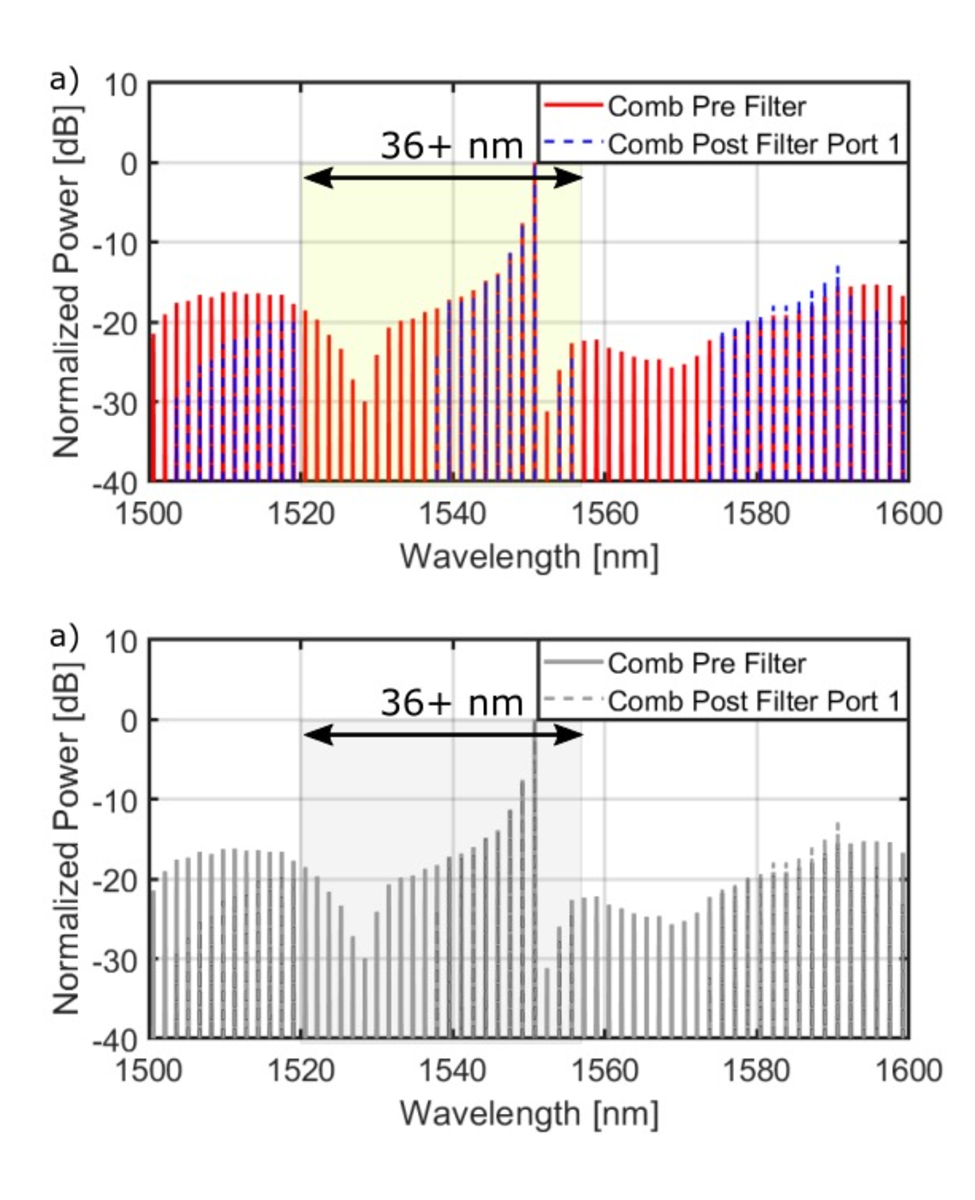
\includegraphics[width=\linewidth]{../../fig/color.pdf}
    \caption{Example of non-robust information encoding solely with color contrast. Top: two spectra distinguishable by people with normal color vision. Bottom: illustrative rendering of the same two spectra possibly perceived by people with color vision deficiency.}
    \label{fig:color}
\end{marginfigure}

\section{Pitfalls and Lessons Learned}
Designing visuals that effectively encode information demands thoughtful consideration and attention to detail, ensuring accessibility for all learners. Drawing from personal experience with minor color vision deficiency, I am acutely aware of the importance of not relying solely on color contrast to convey information. A counter example in Fig.~\ref{fig:color}, where color is the only differentiator between the two spectra, renders the information hard to interpret for those with color vision impairments. The prevalence of color blindness, affecting approximately 8\% of males and 0.5\% of females\footnote{Types of Color Blindness, \url{https://www.colourblindawareness.org/colour-blindness/types-of-colour-blindness/}}, might surprise many. However, this statistic virtually guarantees that in any moderately sized classroom, at least one individual is likely to have some form of color vision deficiency. In recognition of this, I am committed to employing multiple modes of differentiation in my teaching materials, such as patterns, textures, and annotations, to ensure that all students, regardless of visual ability, have equal access to the information presented.

\section{Inclusive Teaching}
Extending beyond color vision awareness, my commitment to inclusivity encompasses all aspects of diversity and accessibility in teaching. I recognize that students come with a broad spectrum of cultural backgrounds, personal experiences, and family education history, all of which impact their learning needs. In light of this, I will strive to create a classroom environment that is not only physically accessible but also cognitively and culturally welcoming. This involves the use of language that is inclusive and bias-free, as well as the incorporation of diverse examples in my teaching materials, for both of which I will conduct regular reflections to ensure compliance.


\section{Teaching Plans}
Aligned with the esteemed curriculum of the \appDept{} at the \appSchool{}, I am eager to contribute by teaching a range of courses that intersect with my expertise,%
\rsCustom{}
\kant[7]

\footnotesize
\nobibliography{\mainabsdir../../common/teaching_statement/bibliography}

\end{document}